\chapter{Design and Implementation}

This chapter presents the architectural and implementation details of Financial Fraud Detection Using Graph Machine Learning. It covers the layered system design, the detection pipeline, data flow across the processing stages, database schemas, the React frontend architecture, and screenshots of the user interface.

\section{Overall Design}
The system follows a \textbf{layered architecture} with clear separation between the client tier, the authentication layer, the API gateway, the detection pipeline, the backend services and persistence. Every request from the single-page application carries a JWT bearer token, which the authentication layer validates before the request reaches a router; the only exceptions are the login endpoint, the health check and a system-information endpoint that returns a configuration flag and no data. Each layer is independently testable and replaceable.

\section{System Design}

\subsection{Database Schema}
All application state is held in a single relational database accessed exclusively through the SQLAlchemy ORM. No module issues raw SQL, so the schema and the queries are expressed once, in the model classes, rather than scattered through the codebase as literal statements.

Row counts are those of the working database at the time of writing: the seeded dataset contributes 5,000 accounts and 80,000 transactions, and the remainder are the accounts and transactions added by hand through the interface while the deployed instance was tested and demonstrated (Section~\ref{sec:dataset}). The \code{alerts} and \code{rule\_hits} counts likewise describe that working database; a fresh run over the seeded data alone produces 2,979 rule hits and, at the default alert threshold of 0.80, 4,134 alerts. Two artefacts of the pipeline are deliberately \textit{not} database tables. The seventeen-column feature matrix is written to \code{data/processed/features.csv}, and the assembled fraud rings are cached to \code{saved\_models/rings.json}; both are derived outputs that are regenerated whenever the pipeline is re-run, so persisting them as relations would duplicate state that the pipeline already owns. Relationships between tables are carried by the business keys (\code{account\_uid}, \code{txn\_uid}, \code{alert\_uid}) rather than by declared foreign-key constraints; the one exception is \code{notification\_reads}, which declares a foreign key on \code{fraud\_notifications.id}. This is a deliberate simplification for a single-process SQLite deployment and is recorded among the limitations in Chapter~\ref{ch:results}.

\begin{table}[htbp]
\centering
\caption{Backend Persistence Schema}
\label{tab:schema}
\footnotesize
\begin{tabularx}{\textwidth}{@{}L{3.6cm}L{1.3cm}Y@{}}
\toprule
\textbf{Table} & \textbf{Rows} & \textbf{Key Columns} \\
\midrule
\code{accounts} & 5,003 & \code{id} (PK), \code{account\_uid} (unique), \code{customer\_name}, \code{email}, \code{phone}, \code{account\_type}, \code{risk\_level}, \code{fraud\_score}, \code{is\_fraud}, \code{review\_status}, \code{created\_at} \\
\code{transactions} & 80,004 & \code{id} (PK), \code{txn\_uid} (unique), \code{sender\_uid}, \code{receiver\_uid}, \code{amount}, \code{timestamp}, \code{txn\_type}, \code{status}, \code{is\_fraud}, \code{fraud\_score} \\
\code{graph\_metrics} & 5,000 & \code{account\_uid}, \code{in\_degree}, \code{out\_degree}, \code{total\_sent}, \code{total\_received}, \code{degree\_centrality}, \code{pagerank}, \code{component\_id}, \code{component\_size}, \code{community\_id}, \code{community\_size}, \code{in\_cycle} \\
\code{alerts} & 4,212 & \code{alert\_uid}, \code{transaction\_uid}, \code{account\_uid}, \code{reason}, \code{fraud\_score}, \code{risk\_level}, \code{status} \\
\code{rule\_hits} & 2,981 & \code{txn\_uid}, \code{rule} --- one row per rule fired on a transaction \\
\code{cases} & variable & \code{case\_uid}, \code{alert\_uid}, \code{account\_uid}, \code{assigned\_to}, \code{notes}, \code{status}, \code{final\_decision} \\
\code{account\_status\_events} & variable & \code{account\_uid}, \code{from\_status}, \code{to\_status}, \code{changed\_by}, \code{transaction\_uid}, \code{note}, \code{created\_at} \\
\code{fraud\_notifications} & variable & \code{kind}, \code{priority}, \code{account\_uid}, \code{transaction\_uid}, \code{amount}, \code{risk\_score}, \code{message} \\
\code{notification\_reads} & variable & \code{notification\_id} (FK), \code{user\_id}, \code{read\_at} \\
\code{email\_deliveries} & variable & \code{kind}, \code{account\_uid}, \code{status\_event\_id}, \code{recipient\_masked}, \code{status}, \code{attempts}, \code{last\_error} \\
\code{users} & 1 & \code{username} (unique), \code{hashed\_password}, \code{role} \\
\code{schema\_migrations} & 3 & \code{version}, \code{applied\_at} --- records the start-up schema upgrades already applied \\
\bottomrule
\end{tabularx}
\end{table}

\begin{figure}[htbp]
\centering
\diagram{architecture}
\caption{High-Level System Architecture}
\label{fig:architecture}
\end{figure}

\subsection{Backend Architecture}
The backend is structured as a Python package (\code{backend/app/}) with clearly separated sub-packages:

\begin{itemize}
  \item \code{api/} --- eighteen FastAPI routers, one per resource: \code{auth}, \code{accounts}, \code{transactions}, \code{preprocessing}, \code{rules}, \code{graph}, \code{features}, \code{ml}, \code{gnn}, \code{alerts}, \code{rings}, \code{cases}, \code{dashboard}, \code{reports}, \code{investigation} (mounted under the \code{/api/accounts} prefix), \code{notifications}, \code{system} and \code{demo}.
  \item \code{ml/} --- the detection modules: \code{rules.py} (rule engine), \code{graph\_build.py} and \code{graph\_analysis.py} (graph metrics), \code{features.py} (feature engineering), \code{baseline.py} (classical model training and scoring), \code{gnn.py} (GCN and GraphSAGE), \code{alerts.py} and \code{fraud\_ring.py}.
  \item \code{services/} --- the response workflow: \code{fraud\_review.py} (analyst decisions and their audit trail), \code{notifications.py} (real-time alerting) and \code{mailer.py} (account-holder email).
  \item \code{demo/} --- the scripted demonstration scenario as pure data, with no database access, so both the planting script and the application can import it.
  \item \code{models/} --- SQLAlchemy declarative models mirroring Table~\ref{tab:schema}, and the Pydantic schemas used for request and response validation.
  \item Root modules --- \code{main.py} holds the application factory and CORS configuration, \code{config.py} the environment-driven settings, \code{database.py} the engine and session factory, \code{deps.py} the authentication and role dependencies, \code{migrations.py} the start-up schema upgrade, and \code{core/security.py} the JWT issuance and password hashing.
\end{itemize}

\subsection{Detection Pipeline Orchestration}
The detection stages are exposed as independent endpoints rather than as a single monolithic job, because each stage has a different cost profile and the analyst needs to be able to re-run one stage without repeating the others. The stages are ordered by dependency: the rule engine reads only the transaction table and can run first; graph analysis builds the NetworkX \code{DiGraph} and persists per-account metrics; feature engineering joins the transaction aggregates with those metrics; model scoring consumes the resulting feature matrix; and the graph neural networks train on the graph and the same feature matrix together. Each endpoint writes its output to the database and returns a summary, so progress survives a page reload and the frontend remains stateless.

The rule engine is also the only writer of an account's risk level. A model score never raises it, which keeps the one field an analyst reads at a glance traceable to a stated rule. A separate \code{onboarding\_risk\_category}, set by hand at customer onboarding, is held apart from it and feeds neither the rules nor the models.

\subsection{Analyst Review and Response}\label{sec:review}
Detection output stops short of a verdict. An account the rules or the models find suspicious is marked \textit{Suspicious}; only an analyst can move it to \textit{Under Review}, \textit{Confirmed Fraud} or back to cleared, and clearing requires a written reason. Three things follow from a confirmation, and the design keeps them consistent:

\begin{itemize}
  \item \textbf{An audit trail.} Every status change writes an \code{account\_status\_events} row recording the analyst, the time, the note and the transaction the decision refers to.
  \item \textbf{An email to the account holder}, queued in the same database transaction as the confirmation, so a confirmation always has exactly one email record --- marked as skipped when the account has no usable address. Repeating a confirmation changes nothing and sends nothing, and clearing an account sends no email at all. Delivery happens after the status is saved, so a mail failure never undoes it; each attempt is logged and can be retried.
  \item \textbf{Real-time alerting.} When a confirmed account sends a further transaction, a high-priority alert and a notification are stored and every open notification stream is woken. The database is the source of truth, so a notification survives a refresh, a new login or a restart, and a client that was disconnected catches up on reconnecting.
\end{itemize}

\subsection{Demonstration Scenario}\label{sec:demo}
A scripted mule-network laundering operation is bundled for demonstrations. Twenty-two accounts and twenty-two transactions, all identified by a \code{DEMO-} prefix, tell a four-stage story chosen so that the complete rule set fires in sequence:

\begin{enumerate}
  \item \textbf{Collection} --- nine feeder accounts pay a mule account opened six days earlier, all within twenty-five minutes (triggers R3 and R4).
  \item \textbf{Consolidation} --- the mule forwards almost the whole balance to a collector in one transfer (R1).
  \item \textbf{Layering} --- collector $\rightarrow$ shell 1 $\rightarrow$ shell 2 $\rightarrow$ collector, each hop deliberately under the reporting threshold (R6).
  \item \textbf{Cash-out} --- nine transfers just under the threshold to nine cash-out accounts within eight minutes (R2 and R5).
\end{enumerate}

The scenario is defined as pure data with no database access, so the planting script and the application share one definition. It can be planted into a copy of the working data or served as a standalone database containing nothing else, which keeps a demonstration from disturbing the real dataset.

\subsection{Frontend Framework (React)}
The React application is built with Vite and follows a hooks-and-service-module pattern:

\begin{itemize}
  \item \textbf{API modules} (\code{api/accounts.js}, \code{api/graph.js}, \code{api/ml.js}, \code{api/alerts.js}, \code{api/cases.js}, \code{api/dashboard.js}, \code{api/reports.js} and their siblings) wrap Axios calls and attach the bearer token through a shared interceptor, so no component constructs a URL or handles a header directly.
  \item \textbf{Pages} (\code{Login}, \code{Dashboard}, \code{Accounts}, \code{AccountDetail}, \code{Transactions}, \code{DataQuality}, \code{RuleDetection}, \code{GraphAnalysis}, \code{Features}, \code{MLScoring}, \code{GNN}, \code{ModelAnalytics}, \code{Alerts}, \code{Notifications}, \code{FraudRings}, \code{Cases}, \code{Reports}, \code{DemoScenario}) hold their own data-fetching state with \code{useState} and \code{useEffect} and render Material UI components.
  \item \textbf{Shared components} provide the application shell, the protected-route wrapper that redirects unauthenticated users to the login page, the money-flow network view, and the Recharts-based chart wrappers used on the dashboard. The shell hides the Model Analytics and Notifications pages from users without an analyst role.
\end{itemize}

\section{Use Case Diagram}\label{sec:usecase}
Figure~\ref{fig:usecase} shows the principal use cases. The application defines three roles --- \code{admin}, \code{analyst} and \code{viewer} (\code{ROLES} in \code{scripts/create\_user.py}) --- but only two permission sets: \code{FRAUD\_ANALYST\_ROLES} in \code{app/deps.py} treats \code{admin} and \code{analyst} identically, so they are drawn as a single actor. Every router requires a signed-in user through \code{get\_current\_user}; a second dependency, \code{require\_fraud\_analyst}, restricts the shaded use cases to that actor. It guards the whole investigation router --- the account investigation record and the review action that marks an account under review, confirms it or clears it, together with the retry of a failed holder email, which is omitted from the diagram for brevity --- as well as the notification endpoints and the graph-neural-network evaluation behind the Model Analytics page.

A \code{viewer} may therefore browse accounts, transactions and graph metrics, run every detection stage including model training, review alerts and fraud rings, and work investigation cases and reports. A viewer cannot open an account's investigation view, change its review status, receive fraud notifications or read the model analytics: the interface hides the Model Analytics and Notifications pages from that role and shows a notice in place of the investigation view, and the API answers 403 if any of them is requested directly. Because the analyst can do everything a viewer can, the Fraud Analyst / Administrator actor is drawn as a specialisation of Viewer, inheriting all of its use cases.

Confirming and clearing are drawn as separate use cases because they behave differently. Every effective confirmation queues exactly one account-holder email in the same database transaction (Section~\ref{sec:review}), so \textit{Confirm fraud} \guillemotleft include\guillemotright s \textit{Notify account holder by email}; whether the queued email is actually delivered depends on the address on file, as the attached note records. Clearing requires a reason and sends nothing, so it has no relationship with the notification. The Account Holder is not a user of the system and initiates none of these actions: they appear only as the secondary actor who receives the notice.

\begin{figure}[htbp]
\centering
\resizebox{\textwidth}{!}{\diagram{usecase}}
\caption{Use Case Diagram}
\label{fig:usecase}
\end{figure}

\section{Context and Data Flow Diagrams}
Figure~\ref{fig:dfd0} shows the system boundary. Figure~\ref{fig:dfd1} decomposes it into the major processes and the data stores they read and write. The detection pipeline itself is shown separately, as a processing flowchart, in Figure~\ref{fig:pipeline}.

\begin{figure}[htbp]
\centering
\diagram{dfd_context}
\caption{Context-Level Data Flow Diagram (Level 0)}
\label{fig:dfd0}
\end{figure}

\begin{figure}[htbp]
\centering
\resizebox{\textwidth}{!}{\diagram{dfd_level1}}
\caption{Level-1 Data Flow Diagram}
\label{fig:dfd1}
\end{figure}

\section{Detection Pipeline Flow}
Figure~\ref{fig:pipeline} shows the order in which the detection stages run and what each one hands to the next. The solid path is the operational pipeline: alert generation reads exactly two upstream signals --- transactions the rule engine marked \code{suspicious}, and accounts whose \code{fraud\_score} the baseline models wrote --- so everything downstream of it depends only on the rule engine and the classical models.

The graph neural networks sit on the dashed branch. They read the same feature matrix and the same graph, but nothing downstream consumes their output: the \code{/api/gnn} router exposes only \code{train}, \code{status} and \code{evaluation}, and \code{alerts.generate()} never reads a GNN score. Training is triggered separately by the analyst, requires PyTorch and PyTorch Geometric, and is unavailable on the free-tier deployment, which does not carry those packages. A complete detection run therefore produces alerts, rings and cases whether or not the graph neural networks have ever been trained.

\begin{figure}[htbp]
\centering
\diagram{pipeline}
\caption{Detection Pipeline Data Flow Diagram}
\label{fig:pipeline}
\end{figure}

\section{Database Design}

\subsection{Entity Relationship Diagram}
Figure~\ref{fig:er} shows the core entities and their relationships, taken from the SQLAlchemy model classes in \code{app/models/}. Underlined attributes are the surrogate integer primary keys; \code{UQ} marks the unique business key each entity is actually referenced by. The relationships shown are those the application maintains in code through those business keys (\code{account\_uid}, \code{txn\_uid}, \code{alert\_uid}); only \code{notification\_reads.notification\_id}, marked \code{FK}, is a foreign key declared to the database. Section~\ref{sec:limitations} records that distinction as a limitation.

\begin{figure}[p]
\centering
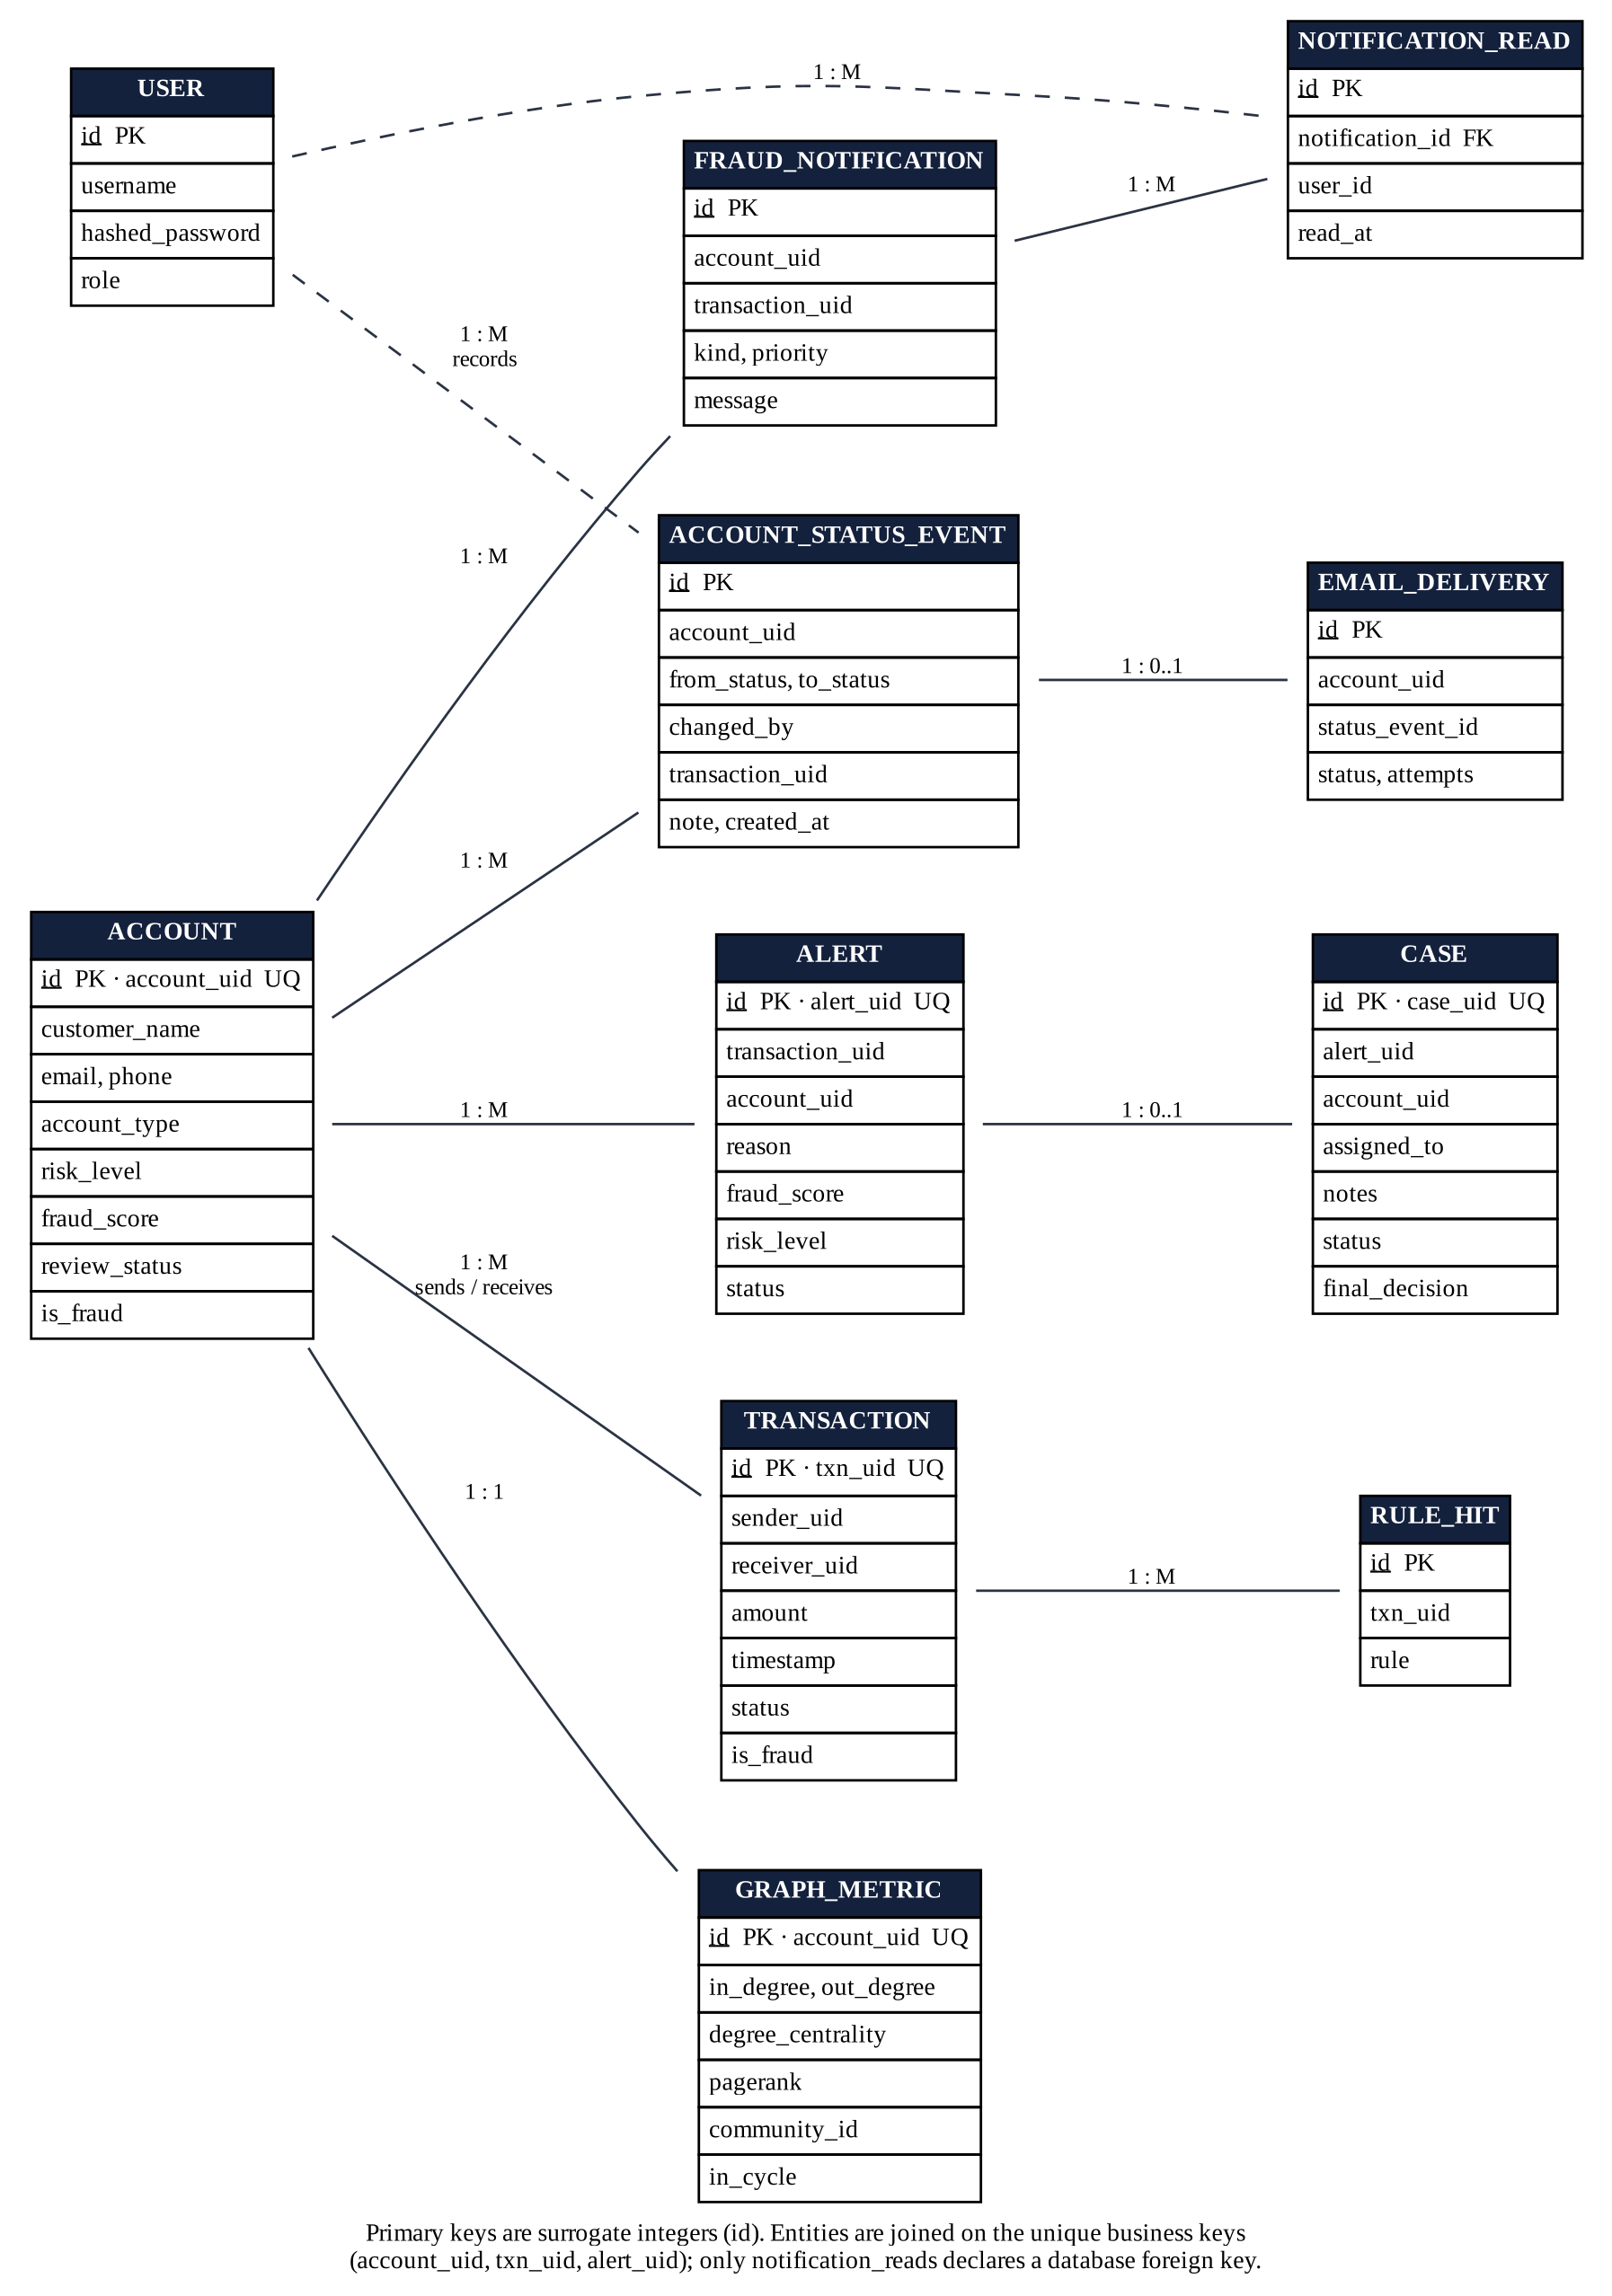
\includegraphics[width=0.97\textwidth,height=0.86\textheight,keepaspectratio]{er_diagram}
\caption{Entity Relationship Diagram}
\label{fig:er}
\end{figure}

\Needspace{28\baselineskip}
\subsection{Table Definitions}

\subsubsection*{Accounts Table}
\begin{lstlisting}[language=SQL, caption={\code{accounts} --- schema as created by the ORM}, label=lst:accounts]
CREATE TABLE accounts (
    id                       INTEGER NOT NULL,
    account_uid              VARCHAR NOT NULL,   -- business key, e.g. ACC00001
    customer_name            VARCHAR NOT NULL,
    email                    VARCHAR,
    phone                    VARCHAR,
    account_type             VARCHAR,            -- Savings | Current | Business | Wallet
    created_at               DATETIME,
    risk_level               VARCHAR,            -- Low | Medium | High (rule engine only)
    fraud_score              FLOAT,              -- model output, 0..1
    is_fraud                 INTEGER,            -- ground-truth label from the dataset
    is_active                INTEGER,
    review_status            VARCHAR,            -- Under Review | Confirmed Fraud | NULL
    review_updated_at        DATETIME,
    fraud_confirmed_by       VARCHAR,
    fraud_confirmed_at       DATETIME,
    onboarding_risk_category VARCHAR,            -- manual KYC category, used by nothing else
    PRIMARY KEY (id)
);
CREATE UNIQUE INDEX ix_accounts_account_uid   ON accounts (account_uid);
CREATE INDEX        ix_accounts_review_status ON accounts (review_status);
\end{lstlisting}

\Needspace{22\baselineskip}
\subsubsection*{Transactions Table}
\begin{lstlisting}[language=SQL, caption={\code{transactions} --- schema as created by the ORM}, label=lst:transactions]
CREATE TABLE transactions (
    id              INTEGER NOT NULL,
    txn_uid         VARCHAR NOT NULL,   -- business key, e.g. TXN0000001
    sender_uid      VARCHAR NOT NULL,   -- -> accounts.account_uid
    receiver_uid    VARCHAR NOT NULL,   -- -> accounts.account_uid
    amount          FLOAT   NOT NULL,
    timestamp       DATETIME,
    txn_type        VARCHAR,            -- transfer | payment | withdrawal
    status          VARCHAR,            -- normal | suspicious (set by the rule engine)
    is_fraud        INTEGER,            -- ground-truth label from the dataset
    fraud_score     FLOAT,
    idempotency_key VARCHAR,            -- guards against duplicate submission
    PRIMARY KEY (id)
);
CREATE UNIQUE INDEX ix_transactions_txn_uid      ON transactions (txn_uid);
CREATE INDEX        ix_transactions_sender_uid   ON transactions (sender_uid);
CREATE INDEX        ix_transactions_receiver_uid ON transactions (receiver_uid);
\end{lstlisting}

\Needspace{18\baselineskip}
\subsubsection*{Alert Record Structure}
A representative row from the \code{alerts} table, serialised as JSON by the API. The values are taken from an actual alert raised during a pipeline run; a \code{null} \code{transaction\_uid} indicates an account-level alert raised from a model score rather than from a single transaction. The score threshold is chosen when alerts are generated (0.50--0.99, default 0.80); this alert was raised in a run that used 0.70.

\begin{lstlisting}[language=json, caption={Alert record as returned by the API (valid JSON)}, label=lst:alert]
{
    "alert_uid":       "ALT000001",
    "transaction_uid": null,
    "account_uid":     "ACC00003",
    "reason":          "ML model: account fraud score 1.00 >= 0.70",
    "fraud_score":     0.9999,
    "risk_level":      "High",
    "status":          "Pending",
    "created_at":      "2026-07-19T17:24:39Z"
}
\end{lstlisting}

\subsubsection*{Account Feature Vector}
\begin{table}[H]
\centering
\caption{Account Feature Vector --- the seventeen columns of \code{FEATURE\_COLS}}
\label{tab:features}
\footnotesize
\begin{tabular}{@{}L{4.2cm}L{1.2cm}L{5.4cm}@{}}
\toprule
\textbf{Field} & \textbf{Type} & \textbf{Description} \\
\midrule
\multicolumn{3}{@{}l}{\textit{Transaction-level features (11)}} \\
\code{total\_sent} & float & Sum of all outgoing amounts \\
\code{total\_received} & float & Sum of all incoming amounts \\
\code{txn\_count\_sent} & int & Number of outgoing transactions \\
\code{txn\_count\_received} & int & Number of incoming transactions \\
\code{unique\_receivers} & int & Distinct accounts paid \\
\code{unique\_senders} & int & Distinct accounts paid by \\
\code{avg\_sent\_amount} & float & Mean outgoing transaction amount \\
\code{avg\_received\_amount} & float & Mean incoming transaction amount \\
\code{max\_sent\_amount} & float & Largest single outgoing transaction \\
\code{max\_received\_amount} & float & Largest single incoming transaction \\
\code{txn\_per\_active\_day} & float & Transactions per day on which the account was active \\
\addlinespace
\multicolumn{3}{@{}l}{\textit{Graph-derived features (6)}} \\
\code{in\_degree} & int & Number of distinct incoming counterparties \\
\code{out\_degree} & int & Number of distinct outgoing counterparties \\
\code{degree\_centrality} & float & Normalised total degree in the account graph \\
\code{pagerank} & float & PageRank score~\cite{page1999} \\
\code{in\_cycle} & int & 1 if the account lies on a directed cycle of length two or three \\
\code{community\_size} & int & Size of the account's Louvain community~\cite{blondel2008} \\
\bottomrule
\end{tabular}
\end{table}

\section{Security Design}
Every control described here was read from the implementation; the section separates what is built from what is not.

\subsection{Authentication and Authorisation}\label{sec:authz}
Login posts an OAuth2 password form to \code{/api/auth/login}. The submitted password is verified against a bcrypt hash held in the \code{users} table, and on success a JSON Web Token is issued, signed with HS256, carrying the username as its subject and expiring after 60 minutes. Protected routes depend on \code{get\_current\_user}, which decodes the token, rejects an invalid or expired signature with 401, and loads the user.

A second dependency, \code{require\_fraud\_analyst}, restricts the sensitive routes to accounts whose role is \code{admin} or \code{analyst} and returns 403 otherwise. It is applied to the whole investigation router --- an account's investigation record, the review action that marks it under review, confirms it or clears it, and the retry of a failed holder email --- to every notification endpoint, and to the graph-neural-network evaluation that backs the Model Analytics page. Every other router depends on \code{get\_current\_user} alone and is open to the \code{viewer} role (Section~\ref{sec:usecase}). The notification stream cannot send an \code{Authorization} header, so it authenticates by token in the query string and the server closes the stream when that token expires.

Two endpoints are deliberately unauthenticated: \code{GET /}, a health check returning a fixed status string, and \code{GET /api/system/info}, which reports whether the instance is running in demonstration mode so the client can hide the training controls. Neither reads the database nor returns any account data.

\subsection{Configuration and Transport}
Secrets --- the token signing key, the administrator password and the SMTP credentials --- are read only from environment variables or a local \code{.env} file. Pydantic is configured with \code{hide\_input\_in\_errors}, so secret values do not appear in validation errors or deployment logs. Unless \code{APP\_ENV} is explicitly set to \code{development}, the application refuses to start if the signing key is a published placeholder, shorter than 32 characters or too repetitive to be random; if the administrator password is the published default or shorter than 12 characters; or if the mail configuration would transmit its password unencrypted. A deployment that omits a variable therefore fails loudly rather than running insecurely.

Cross-origin requests are accepted only from explicitly configured origins, each normalised to \code{scheme://host:port} before comparison. HTTPS is terminated by the hosting platforms; the application does not implement transport security itself. All database access passes through the ORM with bound parameters.

\subsection{Audit Trail and Account-Holder Notification}
Every change to an account's fraud status writes an \code{account\_status\_events} row recording the analyst, the timestamp, the note and the transaction the decision refers to. Each email attempt is logged individually in \code{email\_deliveries} with its outcome.

Confirming an account as fraudulent queues a notice to the account holder. \textbf{This is a demonstration feature, and it would be inappropriate as an automatic action in a real institution}: notifying a suspect that they have been identified can defeat the investigation, and in several jurisdictions disclosure is restricted while a suspicious activity report is pending. In an operational deployment the notice would have to be gated behind an explicit release step authorised by the compliance function, and the system would need to distinguish between a confirmed-fraud victim, who should be told promptly, and a suspected perpetrator, who should not. The implementation here sends to the address on the account without making that distinction.

\subsection{Controls Not Implemented}
The following are absent from the current build and are listed so that the security posture is not overstated: encryption of data at rest (the SQLite file is stored unencrypted); refresh tokens and server-side token revocation (a token is valid until it expires); rate limiting or lockout on repeated failed logins; and multi-factor authentication. No claim of compliance with any banking-sector standard is made or implied.

\section{Screenshots of User Interface}
The following figures illustrate key screens of the analyst web interface. All are static captures of the running application.

\begin{figure}[htbp]
\centering
\begin{subfigure}{0.62\textwidth}\centering
  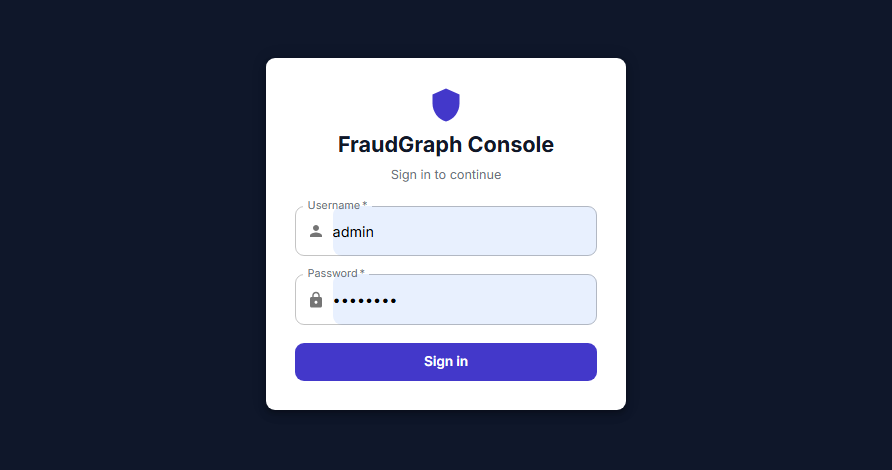
\includegraphics[width=\linewidth]{ui_login}
  \caption{Login Screen --- JWT Authentication}
\end{subfigure}\par\medskip
\begin{subfigure}{\textwidth}\centering
  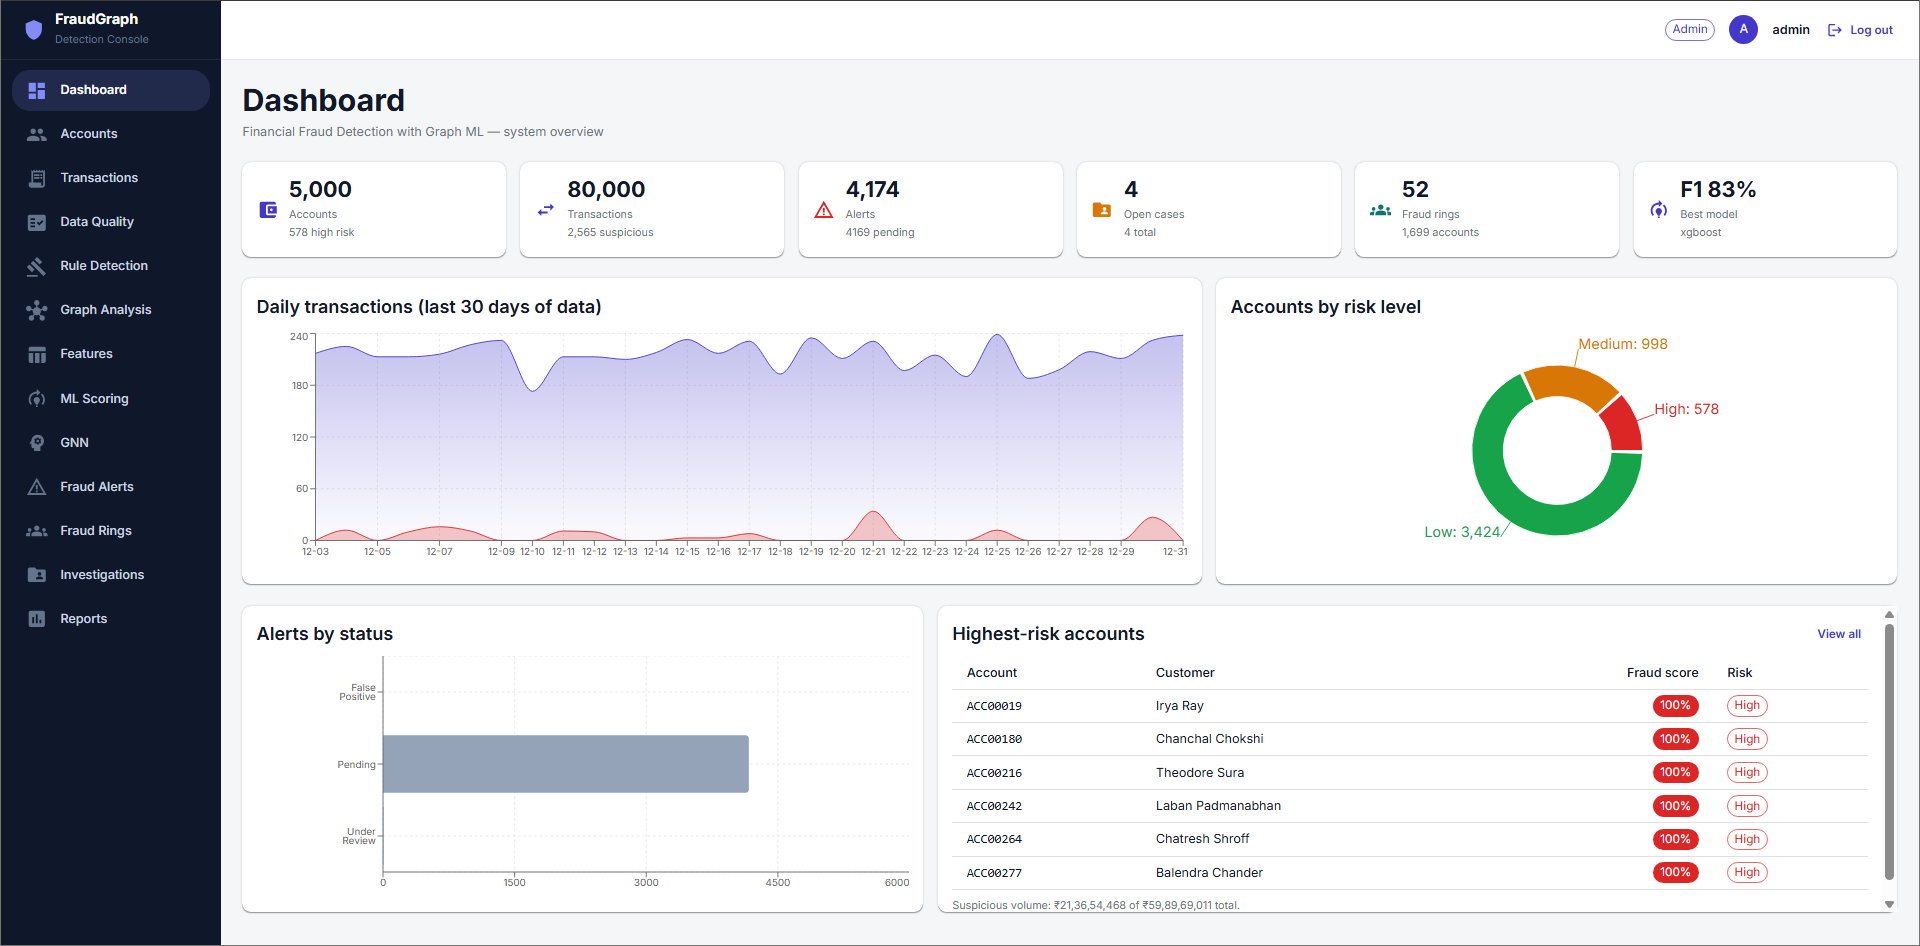
\includegraphics[width=\linewidth]{ui_dashboard}
  \caption{Dashboard --- Portfolio Summary and Risk Distribution}
\end{subfigure}
\caption{User Interface --- Authentication and Dashboard}
\label{fig:ui1}
\end{figure}

\begin{figure}[htbp]
\centering
\begin{subfigure}{\textwidth}\centering
  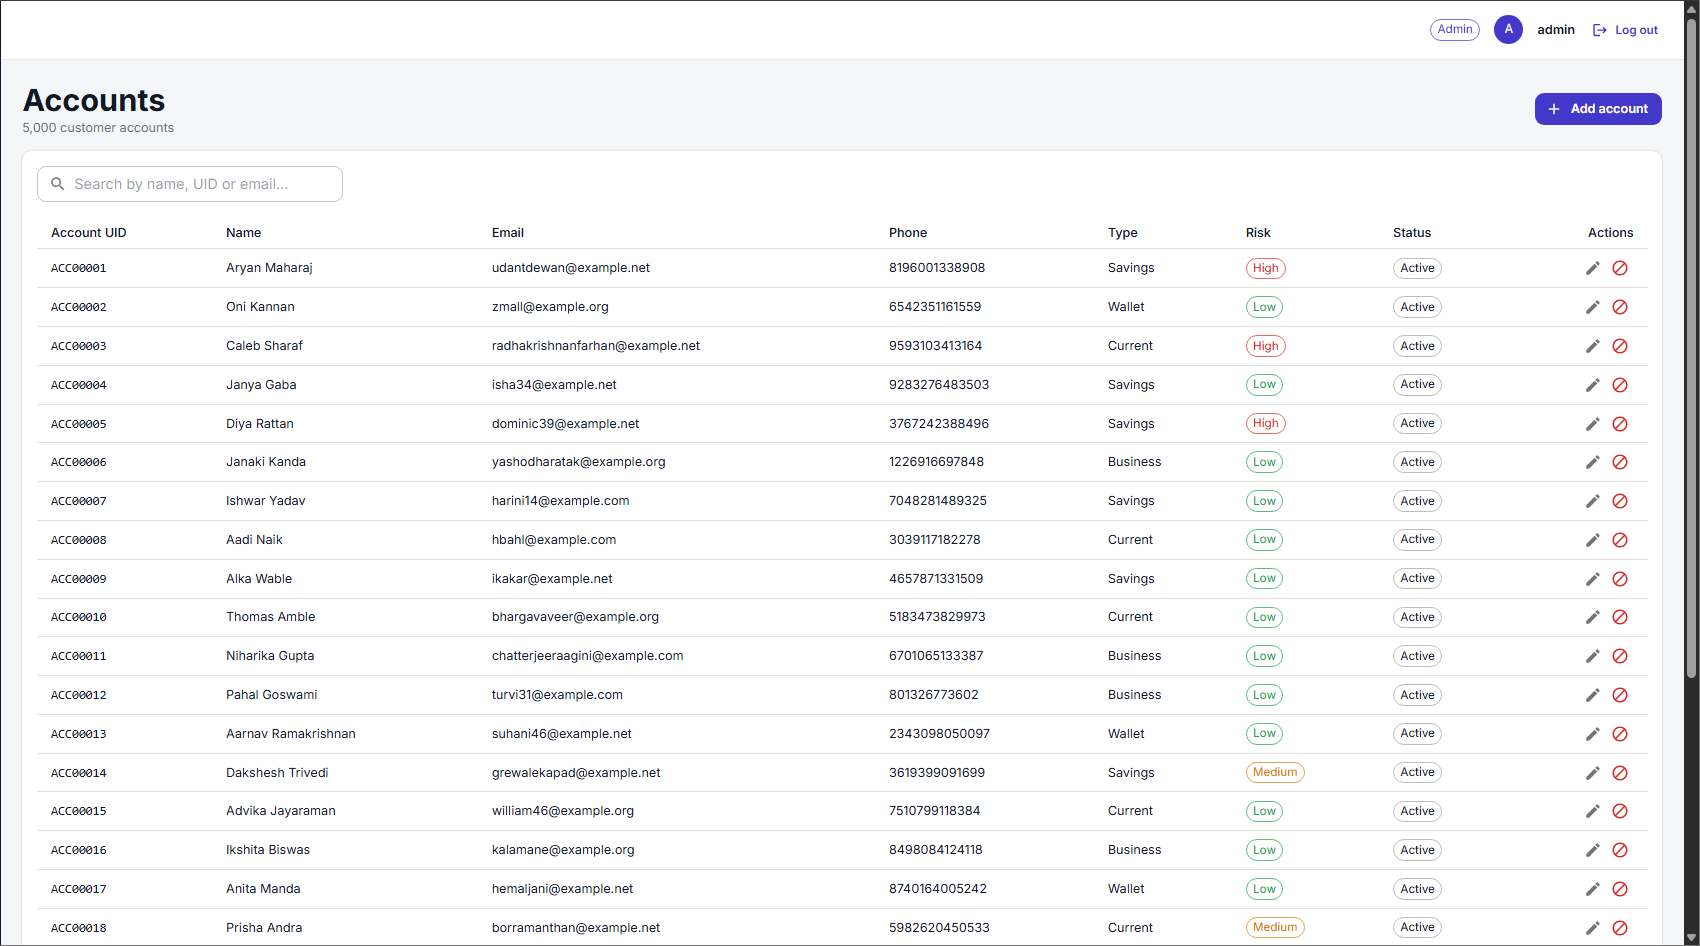
\includegraphics[width=\linewidth]{ui_accounts}
  \caption{Accounts View --- Searchable Account Register with Risk Levels}
\end{subfigure}\par\medskip
\begin{subfigure}{\textwidth}\centering
  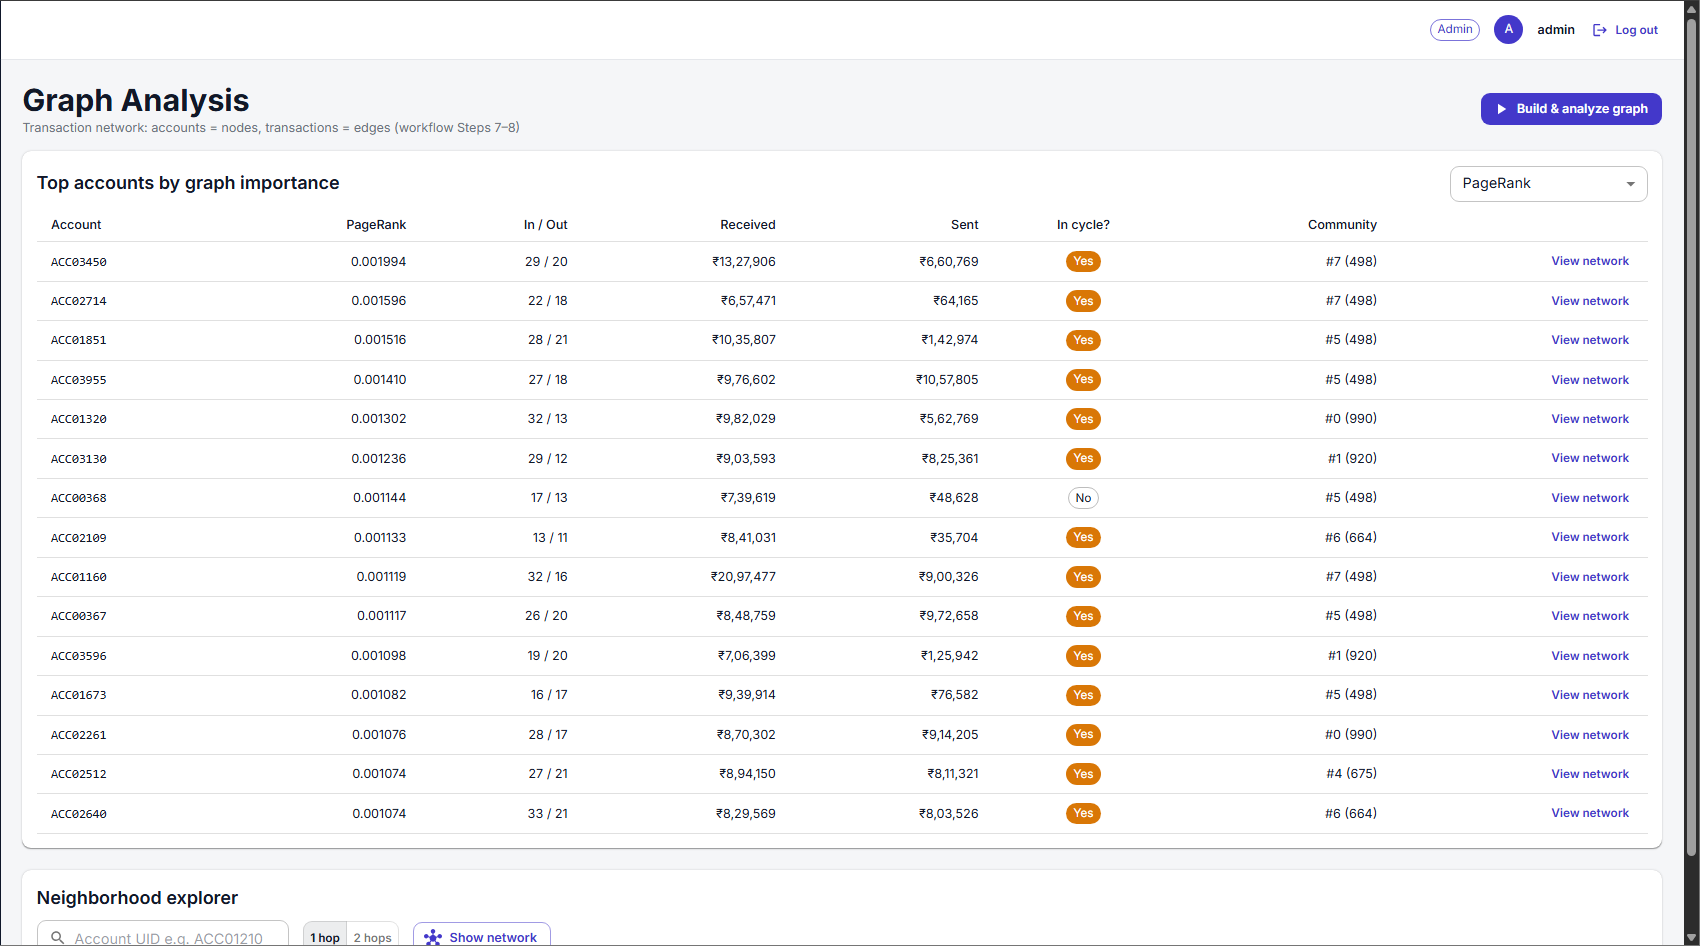
\includegraphics[width=\linewidth]{ui_graph_analysis}
  \caption{Graph Analysis --- accounts ranked by graph importance, with a neighbourhood explorer for a selected account}
\end{subfigure}
\caption{User Interface --- Accounts and Graph Analysis}
\label{fig:ui2}
\end{figure}

\begin{figure}[htbp]
\centering
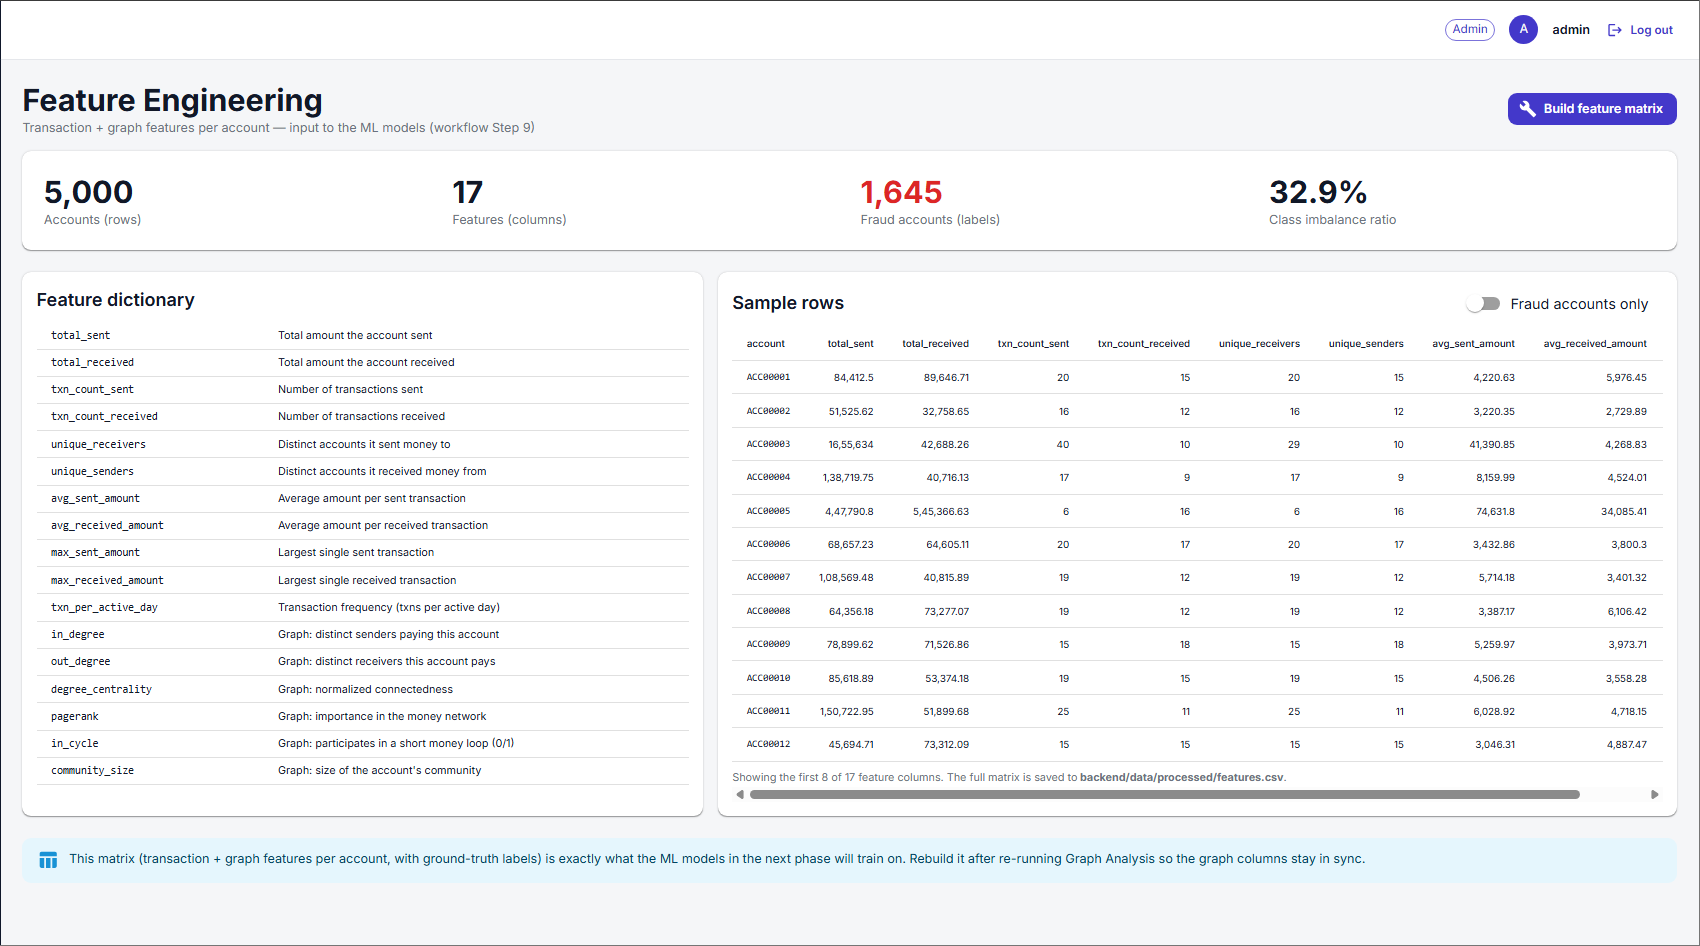
\includegraphics[width=\textwidth]{ui_features}
\caption{Feature Engineering View --- Per-Account Feature Matrix and Model Scores}
\label{fig:ui3}
\end{figure}

\begin{figure}[htbp]
\centering
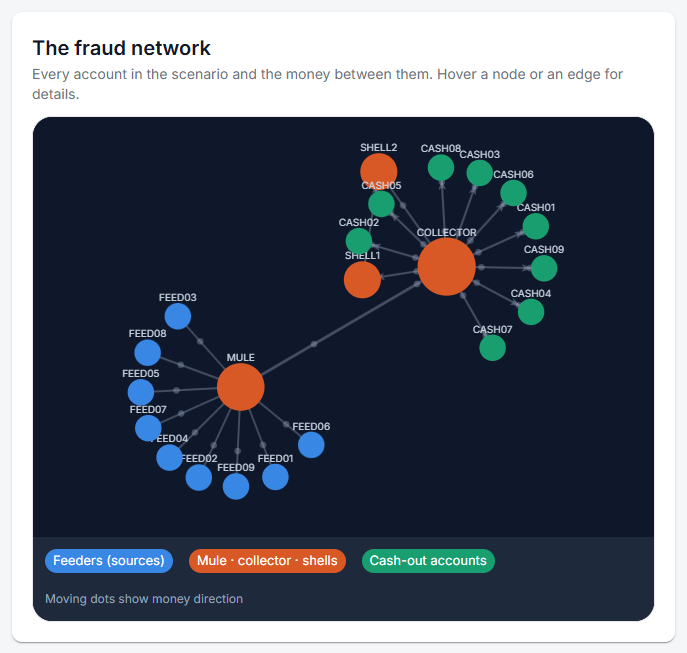
\includegraphics[width=0.62\textwidth]{ui_demo_network}
\caption[Demonstration Scenario --- static screenshot of the interactive money-flow network of Section~\ref{sec:demo}]{Demonstration Scenario --- static screenshot of the interactive money-flow network for the scripted twenty-two-account scenario of Section~\ref{sec:demo}, with the feeders, the mule and collector, the two shell accounts and the nine cash-out accounts coloured by role. Arrowheads at the receiving end of each edge mark the direction of money flow; in the running application dots also travel along the edges in that direction, and the small dots visible on the edges here are those markers captured at one instant}
\label{fig:ui4}
\end{figure}

\begin{figure}[htbp]
\centering
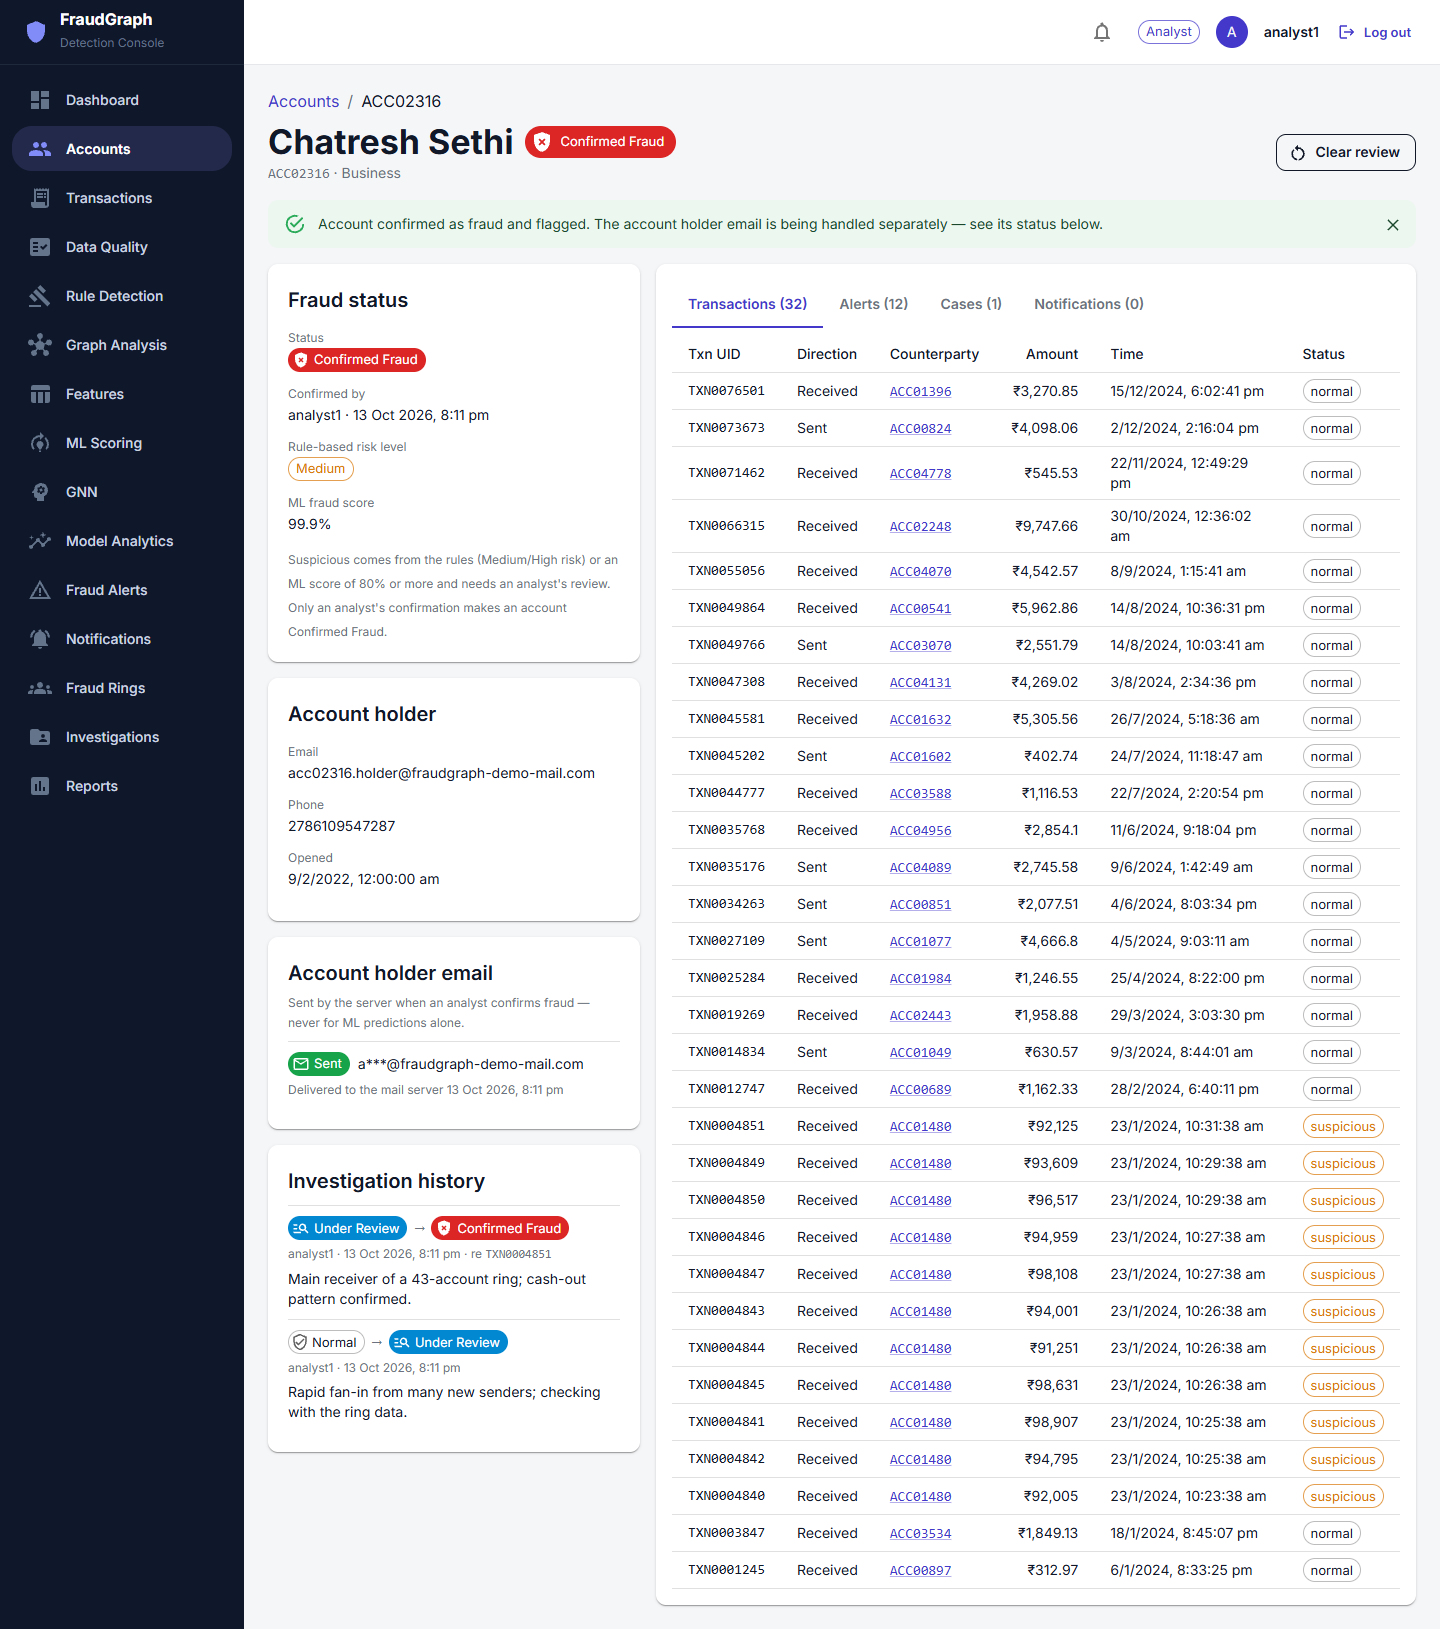
\includegraphics[width=\textwidth,height=0.80\textheight,keepaspectratio]{ui_account_investigation}
\caption{Account Investigation --- a confirmed fraud account showing the analyst and timestamp that confirmed it, the rule-based risk level alongside the independent model score, the account-holder notification that was sent on confirmation with the recipient address masked, the audit trail of status transitions with the analyst's notes, and the account's suspicious transactions}
\label{fig:ui5}
\end{figure}
